\documentclass[border=10pt]{standalone}

\usepackage{tikz}
\usepackage{tikzsymbols}
\usetikzlibrary{calc,patterns,shapes.geometric}

\def\centerarc[#1](#2)(#3:#4:#5){\draw[#1] ($(#2)+({#5*cos(#3)},{#5*sin(#3)})$) arc (#3:#4:#5);}

\begin{document}
	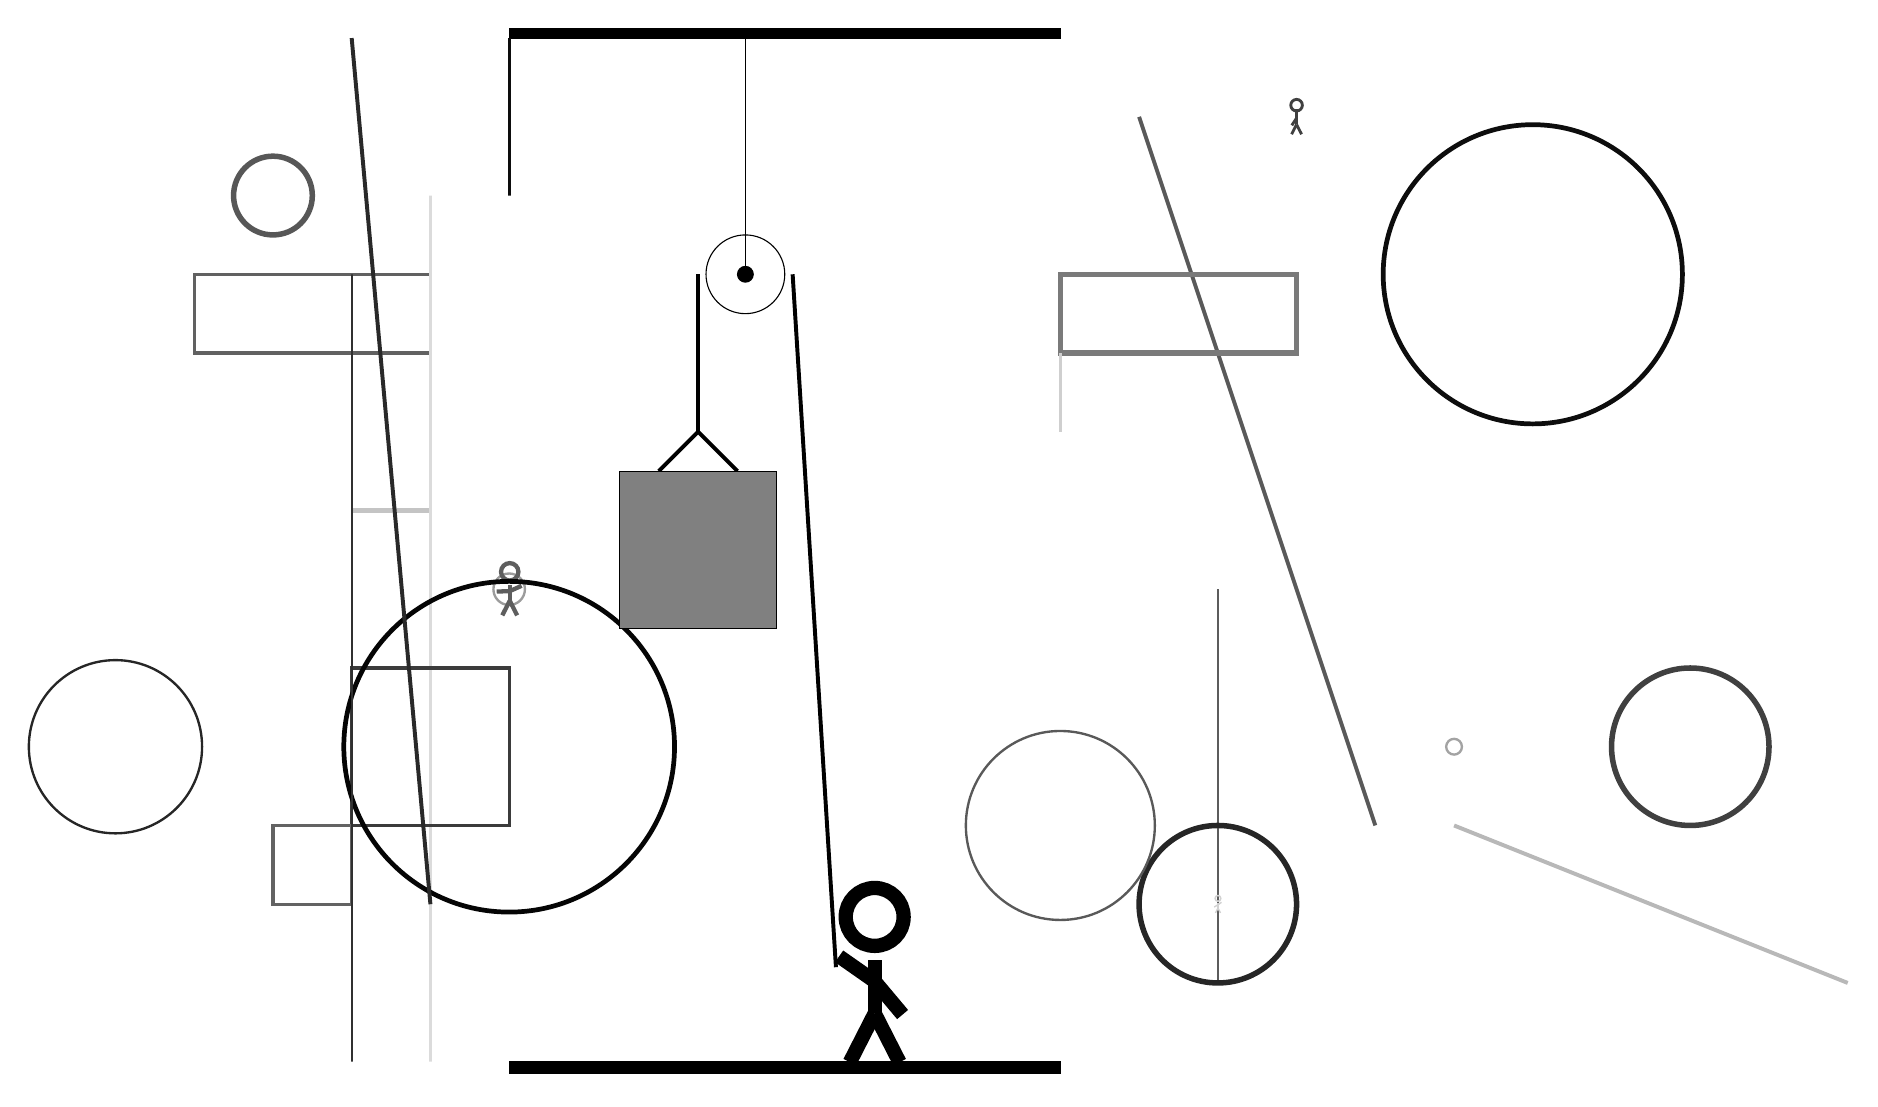
\begin{tikzpicture}
		%%%%% START %%%%%
		
		\draw[fill=black] (-2, 10) rectangle (5, 10.125);
		
		\draw (1, 7) circle (0.5);
		\draw[fill=black] (1, 7) circle (0.1);
		\draw (1, 10) -- (1, 7);
		
		\draw[line width=0.5mm, color=black!65](6, 9) -- (9, 0);
		
		\draw [line width=0.7mm, color=black!66](-5, 8) circle (0.5);
		\draw [line width=0.7mm, color=black!75](13, 1) circle (1.0);
		\draw[line width=0.4mm, color=black!62] (-3, 6) rectangle (-6, 7);
		
		\draw [line width=0.3mm, color=black!39](-2, 3) circle (0.2);
		\draw[line width=0.4mm, color=black!95] (-2, 8) rectangle (-2, 10);
		\draw[line width=0.3mm, color=black!64] (7, -2) rectangle (7, 3);
		\draw[line width=0.7mm, color=black!52] (5, 7) rectangle (8, 6);
		\draw[line width=0.6mm, color=black!23] (-4, 4) rectangle (-3, 4);
		\draw[line width=0.4mm, color=black!14] (-3, 8) rectangle (-3, -3);
		\draw [line width=0.7mm, color=black!85](7, -1) circle (1.0);
		\node[line width=0.2mm, color=black!75] at (8, 9) {\Strichmaxerl[2][57][90]};
		\draw [line width=0.3mm, color=black!65](5, 0) circle (1.2);
		
		\draw [line width=0.3mm, color=black!36](10, 1) circle (0.1);
		\draw[line width=0.5mm, color=black!28](10, 0) -- (15, -2);
		\node[line width=0.5mm, color=black!63] at (-2, 3) {\Strichmaxerl[3][2][24]};
		
		\draw[line width=0.4mm, color=black!77] (-2, 2) rectangle (-4, 0);
		\draw[line width=0.4mm, color=black!19] (5, 5) rectangle (5, 6);
		\draw[line width=0.4mm, color=black!61] (-4, 0) rectangle (-5, -1);
		\draw [line width=0.6mm, color=black!98](-2, 1) circle (2.1);
		\draw[line width=0.5mm, color=black!84](-3, -1) -- (-4, 10);
		
		\node[line width=0.5mm, color=black!18] at (7, -1) {\Strichmaxerl[1][30][36]};
		\draw [line width=0.3mm, color=black!85](-7, 1) circle (1.1);
		\draw[line width=0.3mm, color=black!81] (-4, 7) rectangle (-4, -3);
		\draw [line width=0.6mm, color=black!95](11, 7) circle (1.9);
		
		
		\draw[line width=0.5mm] (-0.1, 4.5) -- (0.4, 5.0) -- (0.9, 4.5);
		\draw[fill=black!50] (-0.6, 4.5) rectangle (1.4, 2.5);
		
		\draw[line width=0.5mm] (0.4, 7) -- (0.4, 5.0);
		\centerarc[line width=0.5mm](1, 7)(0:180:0.6);
		\draw[line width=0.5mm](1.6, 7) -- (2.15, -1.8);
		
		\node at (2.6, -1.9) {\Strichmaxerl[10][-35][-50]};
		
		\draw[fill=black] (-2, -3) rectangle (5, -3.15);
		
		%%%%% END %%%%%
	\end{tikzpicture}
\end{document}